\section{Morphology and spectrum of the gamma-ray emission at the base of the FB}


\subsection{Latitude profiles}
\label{sec:Latitude_profiles}

In order to quantitatively estimate the difference in the intensity of emission of the FB at high latitudes and at the base as well as the asymmetry
of the gamma-ray emission at the base of the FB,
we plot the latitude profiles to the left and to the right of the GC.
In Figure \ref{fig:Profiles} we show the profiles of SED integrated in the energy range $10 - \SI{100}{GeV}$ as a function of Galactic latitude
for different models of Galactic foreground emission.
%The regions have a width of $\ang{4}$ for $|b|<\ang{10}$ and $\ang{10}$ for $|b|>\ang{10}$ in latitude and a width of $\ang{10}$ in longitude. 
%that is $\ang{0} - \ang{10}$ to the East of the GC an $\ang{-10} - \ang{0}$ to the West of the GC. 
%The profiles of the three models include the residual emission plus the FB, i.e. 
For the low-energy model, the profiles show the residual, for the rectangles model -- the sum of residual and rectangles template, 
and for the GALPROP model --  the sum of residual, FB template and GC excess template, as described in Section \ref{sec:Modeling}. 
For comparison we show the latitude profile of the total gamma-ray data outside of the PS mask.
%We observe an agreement between all models and a East-West assymmetry close to the GC. 
For positive longitudes,
some models overpredict the gamma-ray data which leads to negative residuals.
For negative longitudes there is an increase of flux in the Galactic plane by at least a factor of 2 for all models relative to the gamma-ray emission
from the FB at high latitudes. 
The residual of the GALPROP model differs from the low-energy and rectangles model in the Galactic plane by a factor of 2 to 3. 
This may be due to additional freedom in the GALPROP model related to the usage of many templates in the Galactic plane,
the inability of the GALPROP templates to fit the data is also manifested by the negative residuals to the East of the GC.
%Also the data shows a slight East-West assymmetry in the flux around the GC.


\begin{figure*}[h]
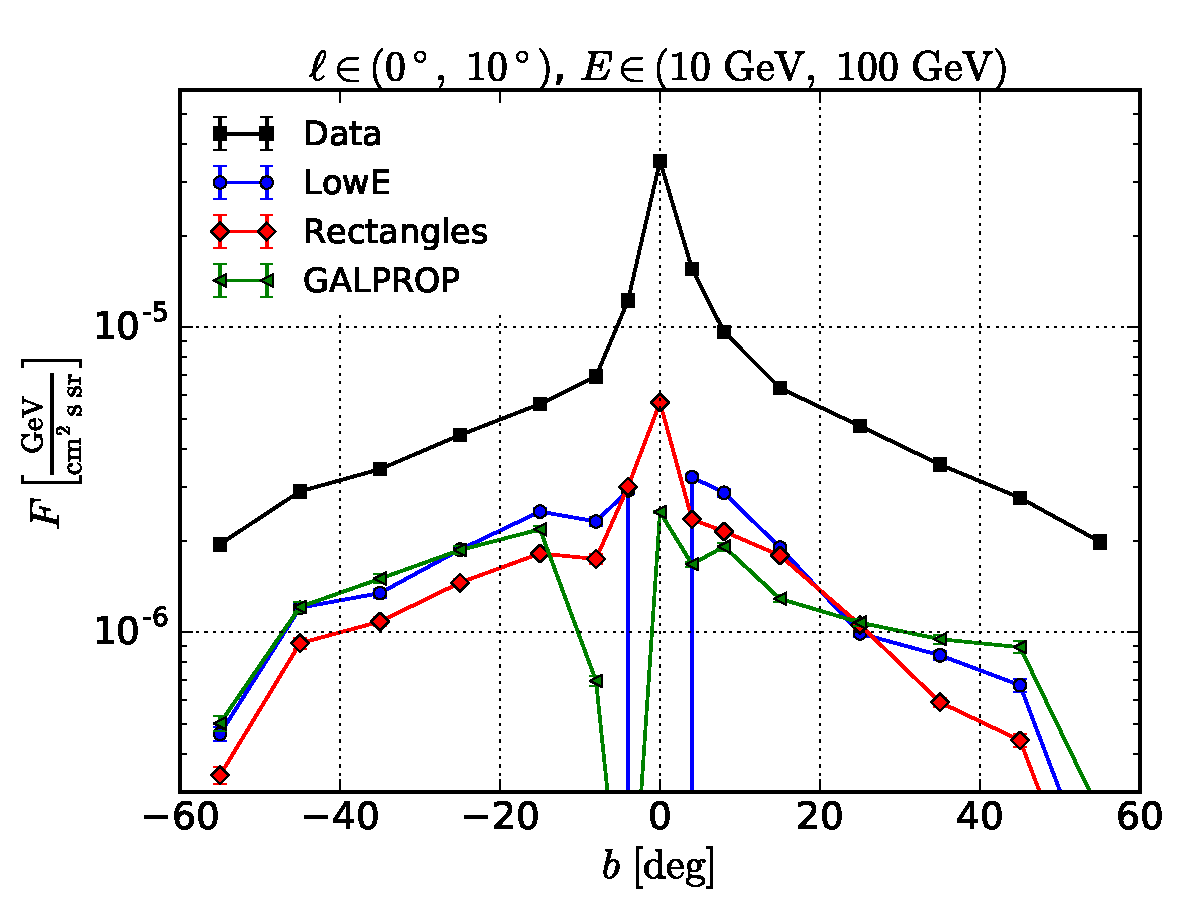
\includegraphics[width=0.5\textwidth]{plots/Profiles_l=1_source_range_1.pdf}
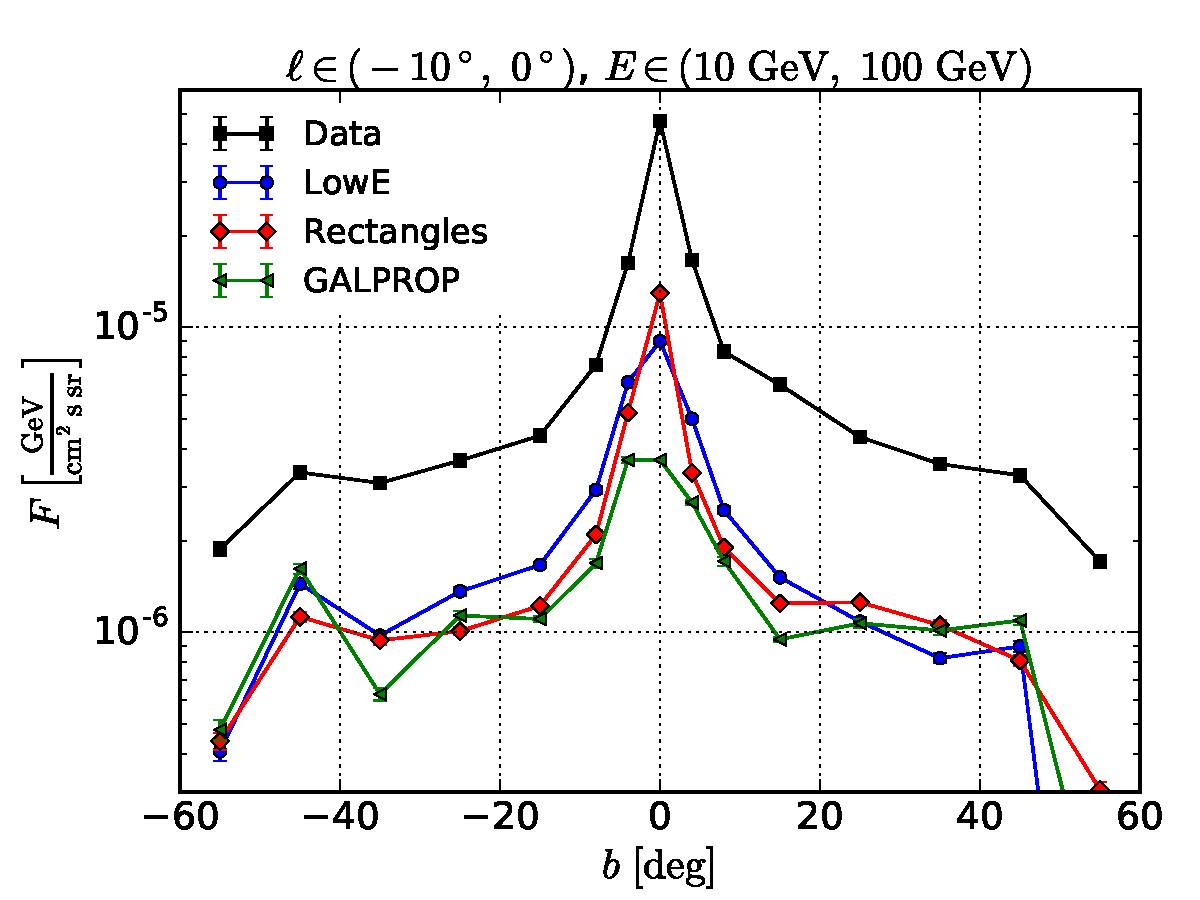
\includegraphics[width=0.5\textwidth]{plots/Profiles_l=0_source_range_1.pdf}
  	\caption{Latitude profiles of the different model residals and the data with PS mask in 
	the units of flux integrated between 10 and 100 GeV to the east (left) and to the west (right) of the GC.}
  	\label{fig:Profiles}
\end{figure*}

\subsection{Comparison of the spectra at different latitudes}

\begin{figure*}[h]
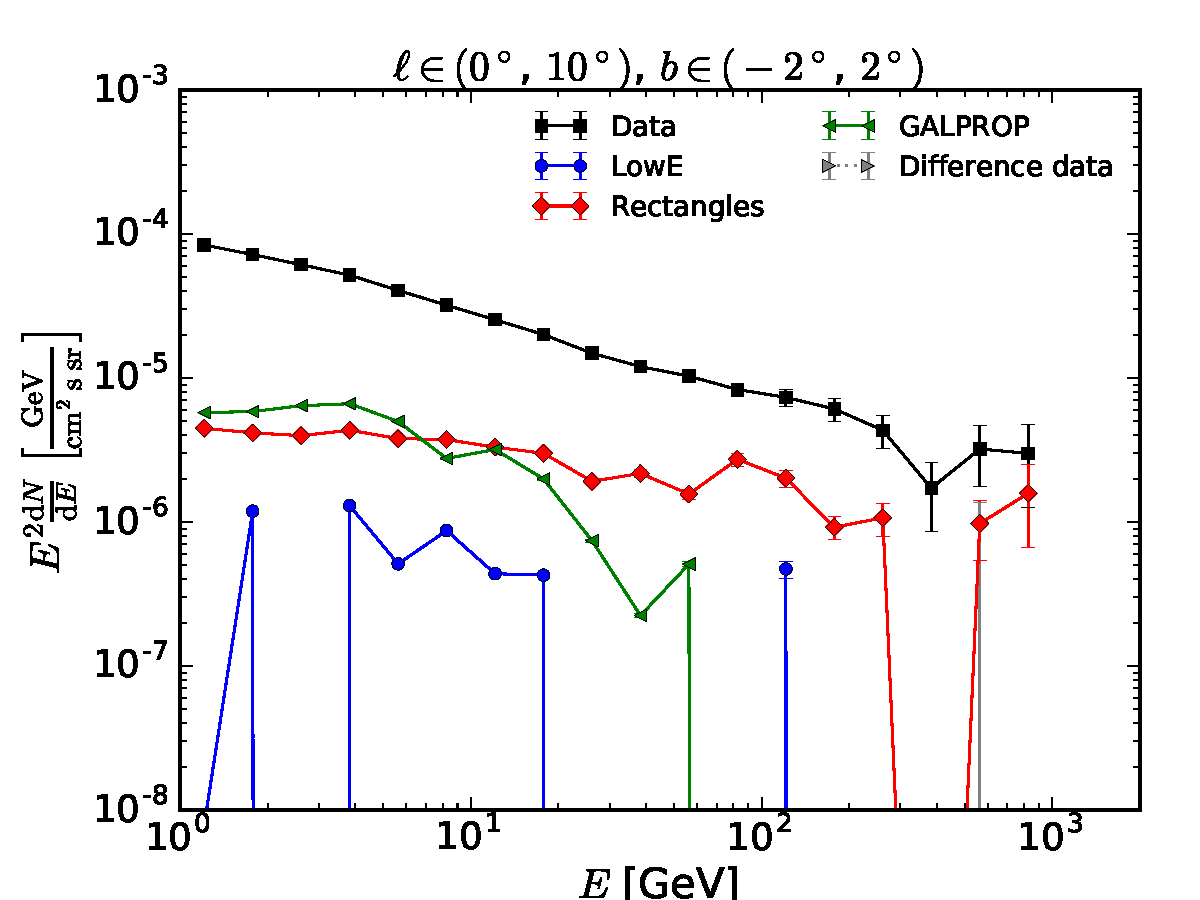
\includegraphics[width=0.5\textwidth]{plots/SED_all_models_source_l=5_b=0.pdf}
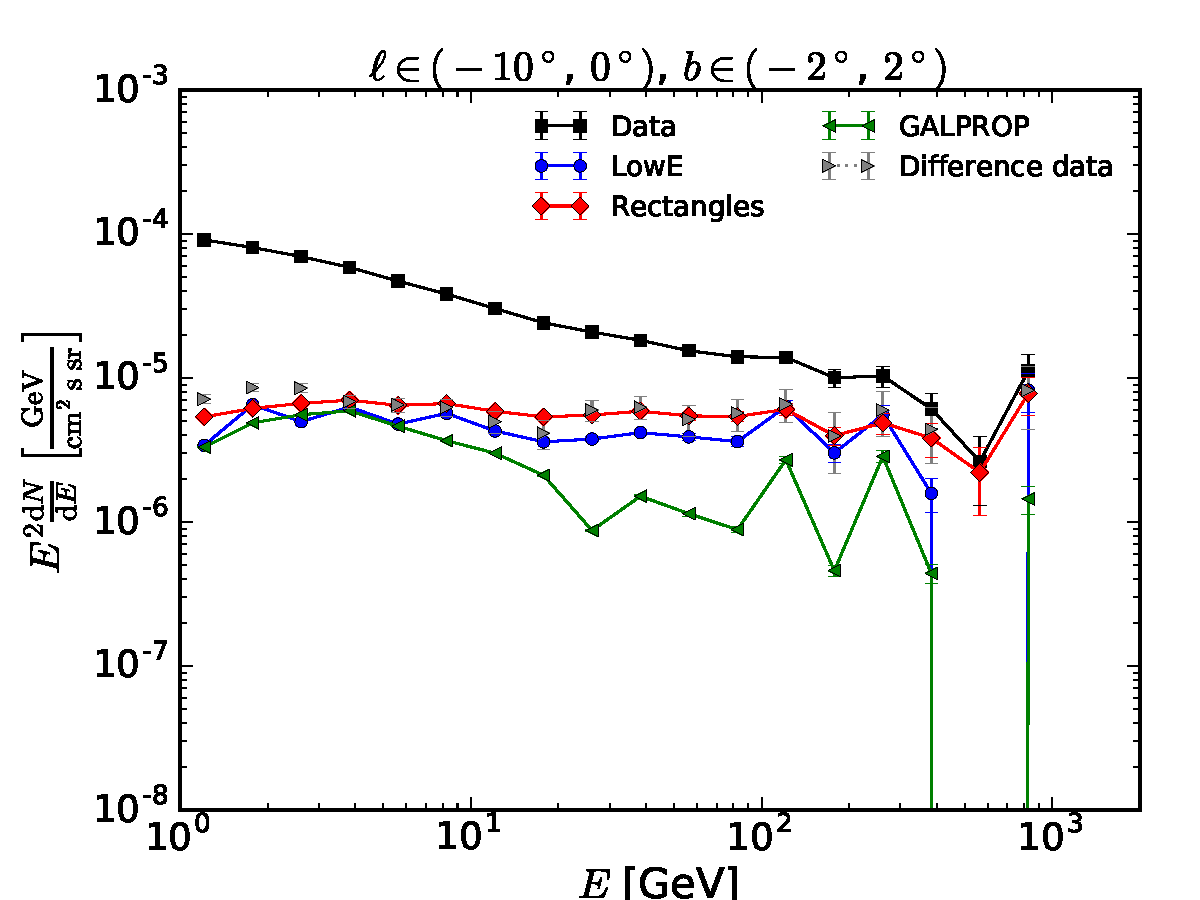
\includegraphics[width=0.5\textwidth]{plots/SED_all_models_source_l=-5_b=0.pdf}
  	\caption{SED of the model residuals, the data with PS mask and the difference in the data with PS mask West minus East. The width of the regions in longitude is $\ang{10}$, i.e. $\ang{0}$ to $\ang{10}$ to the East of the GC (left) and $\ang{-10}$ to $\ang{0}$ to the West of the GC (right).}
  	\label{fig:SED_all}
\end{figure*}

In this section we quantify the hardening of the gamma-ray spectrum at the base of the FB. 
We first compare the SED of the residuals plus the FB models for different foreground models in Figure \ref{fig:SED_all}. 
The differential flux is averaged over regions to the east, $\ell \in (\ang{0},\ \ang{10})$, and to the west, $\ell \in (\ang{-10},\ \ang{0})$, of the GC
in a thin stripe covering the Galactic plane $b \in (\ang{-2},\ \ang{2})$. 
For comparison, we show the data with PS mask and, on the plot for $\ell \in (\ang{-10},\ \ang{0})$, the difference in the data west minus east
of the GC.

For negative longitudes, all models give similar results. 
The differential flux of the GALPROP model is smaller than the differential flux of the other models above 10 GeV, 
which is consistent with the profile plots in Figure \ref{fig:Profiles}.
We also find an asymmetry in the flux of the data with PS mask. The difference of the data West minus East is similar to the flux of the low-energy and rectangles models. The spectra at positive longitudes show large oversubtractions and an overall softer spectrum. %\Laura{Should we show here the plots for (-6,-2) and (2,6) deg latitude also?}
%\dima{I'm not sure, it will take space}

To compare the behavior of the energy spectra at high energies for different latitudes, 
we fit a log-parabola

 \be
 f(E) = N_0 \left(\frac{E}{\SI{1}{GeV}}\right)^{-\alpha - \beta \ln(E)}
 \ee
in each latitude stripe. The local ``index'' of the spectrum at energy $E$ is

\be 
\lb{eq:log_par}
n \equiv - \frac{\de \ln f}{\de \ln E} = \alpha + 2 \beta \ln\left(\frac{E}{\SI{1}{GeV}}\right).
\ee
In Figure \ref{fig:logpar_index} we compare this log-parabola index $n$ as a function of latitude at $E = \SI{500}{GeV}$. 
%\Laura{You called it bubble! ;)} \dima{bubble removed}
We plot $(2 - n)$, which corresponds to the SED index.
For positive longitudes the index is relatively soft ($n > 2$) for most of the latitudes, 
except high latitudes where the gamma-ray statistics is small.
For negative longitudes the index near the GC
is significantly harder ($n \approx 2$) than the index at higher latitudes.
%\Laura{Would you like the x-axis of the log-par plot to show n-2?}
%\dima{yes, I'd suggest to put (2 - n) on the y-axis}
\begin{figure*}[h!]
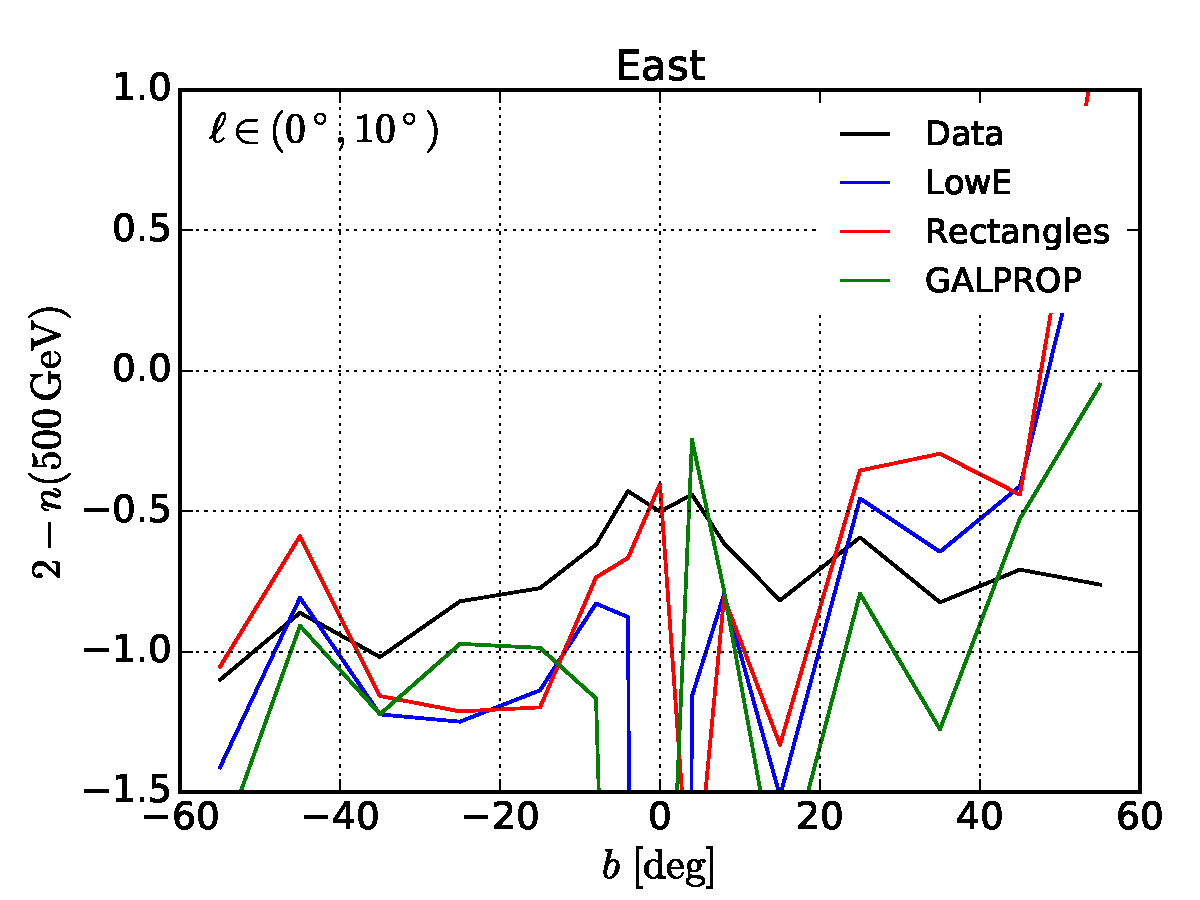
\includegraphics[width=0.5\textwidth]{plots/LogParabola_n(500GeV)_l_in_(0,10).pdf}
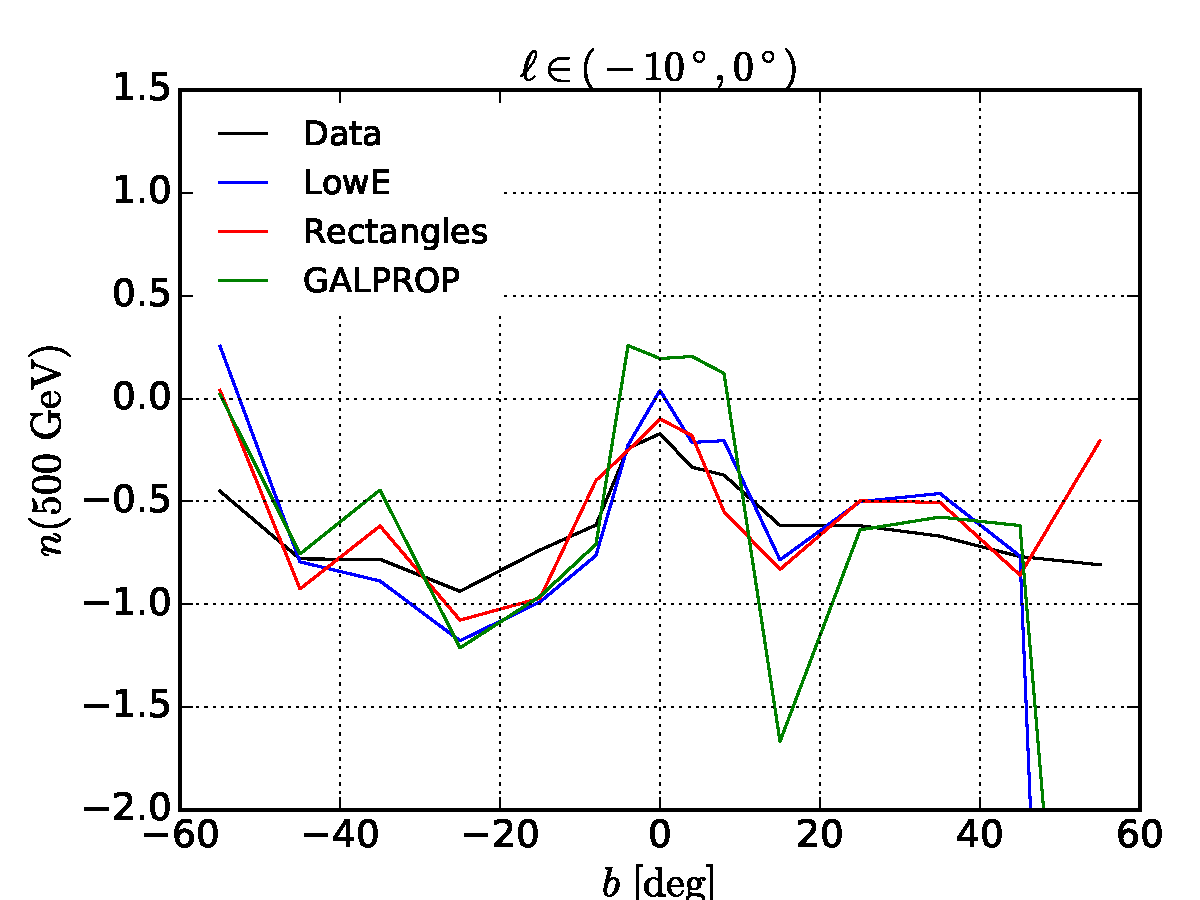
\includegraphics[width=0.5\textwidth]{plots/LogParabola_n(500GeV)_l_in_(-10,0).pdf}
\caption{Index of the log-parabola (Equation (\ref{eq:log_par})) at  $E = \SI{500}{GeV}$ as a function of latitude for residuals in 
the different foreground diffuse models. 
%The width of the regions in longitude is $\ang{10}$, i.e. $\ang{0} - \ang{10}$ to the East of the GC (left) and $\ang{-10} - \ang{0}$ to the West of the GC (right).
}
\label{fig:logpar_index}
\end{figure*}


\subsection{Parametric model of the gamma-ray spectrum at low latitudes}
\label{sec:param_model}

In this section we study in detail the spectrum of the FB at latitudes $|b| < 6^\circ$.
As a baseline model we use the rectangles model of the FB.
We compare a power-law model of the energy spectrum with a power-law and an exponential cutoff model.
For the model with a cutoff, we find the 95\% statistical confidence interval for the cutoff energy 
(we report the lower boundary of the interval).
At last, we find the minimum among the 95\% confidence levels for all considered models.
The results are summarized in Table \ref{tab:param}.
The spectrum of the residuals including the FB at  $\ell \in (\ang{-10},\ \ang{0})$
is consistent with a power law with an index $2.1 - 2.2$ and without a cutoff up to $E \approx 1$ TeV.
\dima{Report the total luminosity (assuming the GC location) in erg/s including modeling ``error bars", 
we can also do it in Section \ref{sec:GC_scenario}.}

\begin{table*}
  \begin{center}
    \caption{Parametric model of the FB. We report the best fit values of the spectrum, the significance of the cutoff, 
    and statistical 95\% confidence on $E_{\rm cut}$ for the rectangles model.
    The last column is the minimum among all models of the 95\% statistical confidence value of $E_{\rm cut}$.
    \dima{I'm curious why the rectangles model is also the min model for negative longitudes.}}
    \label{tab:param}
    \begin{tabular}{|c|c|c|c|c|c|c|c|} % <-- Alignments: 1st column left, 2nd middle and 3rd right, with vertical lines in between
     	\hline
		 Lat & Lon  & norm & index & cutoff &  $-2 \Delta \log \La$ & cutoff 95\% stat & cutoff 95\% min \\ 
		       &        &  $\SI{e-6}{\frac{GeV}{cm^{2}s\ sr}}$ &  & $\SI{}{GeV}$ & & $\SI{}{GeV}$ & $\SI{}{GeV}$ \\ 
		\hline
  		$(\ang{2}, \ang{6})$ & $(\ang{0}, \ang{10})$ & 1.9  & 1.9 & 45 & 4.8 & 25 & 25 \\ 
		& $(\ang{-10}, \ang{0})$ & 2.0  & 2.2 & -- & 0.0 & \Laura{308} & \Laura{308}  \\ 
 		\hline
  		$(\ang{-2}, \ang{2})$ & $(\ang{0}, \ang{10})$  & 3.5  & 2.3 & -- & 0.0 & \Laura{210} & 2.4  \\ 
		& $(\ang{-10}, \ang{0})$  & 6.4  & 2.1 & -- & 0.0 & \Laura{350} & \Laura{350}   \\ 
 		\hline
  		$(\ang{-6}, \ang{-2})$ & $(\ang{0}, \ang{10})$  & 1.8  & 2.1 & 260 & 3.8 & 120 & 11  \\ 
		& $(\ang{-10}, \ang{0})$ & 2.8  & 2.2 & -- & 0.0 & \Laura{330} & \Laura{330} \\ 
 \hline
    \end{tabular}
  \end{center}
\end{table*}




\subsection{IC model of the gamma-ray emission}
\label{sec:IC_model}

In this section we model the gamma-ray emission at the base of the FB via the IC scattering.
As a baseline case, we take the gamma-ray spectrum derived in the rectangles model of the FB in Section \ref{sec:box_model}.
The source function for the IC gamma-rays is

\be
\label{eq:IC_spectrum}
E_\g\frac{\de Q_{\rm IC}}{\de E_\g} = c\int\!\! \int \left(\frac{\de n}{\de E}\right)_{\!\!\ISRF} \sigma_\IC\ \left(\frac{\de n}{\de E}\right)_{\!\!\el} \de E_\ISRF\, \de E_\el,
\ee
where $(\de n/ \de E)_\ISRF\ [\SI{}{GeV^{-1} cm^{-3}}]$ is the number density of ISRF photons,
$(\de n / \de E)_\el\ [\SI{}{GeV^{-1} cm^{-3}}]$ is the number density of electrons, and $\sigma_\IC(E_\gamma, E_\ISRF, E_\el)$
is the differential IC scattering cross section in units of $E_\g\frac{d\sigma}{d E_\g}$ \citep{1970RvMP...42..237B}.
The ISRF number density for starlight and IR photons is taken from GALPROP v54.
For the CMB, we use the thermal spectrum with the temperature $\SI{2.73}{K}$.
The SED intensity of gamma rays is

\be
E^2 \frac{dF}{dE} = \frac{1}{4 \pi} \int E^2\frac{\de Q}{\de E} dR = 
\frac{Ec}{4\pi}\int \int \left(\frac{\de n}{\de E}\right)_{\!\!\ISRF} \sigma_\IC\ \left(\frac{\de \Sigma}{\de E}\right)_{\!\!\el} \de E_\ISRF\, \de E_\el,
\ee
where $\left(\frac{\de \Sigma}{\de E}\right)_{\!\!\el} = \int \left(\frac{\de n}{\de E}\right)_{\!\!\el} dR$ is the column density 
of CR electrons.
We will model the column density of electrons as a power law with a cutoff

\be 
\label{eq:e_spectrum}
\left(\frac{\de \Sigma}{\de E}\right)_{\!\!\el} = n_\el \left(\frac{E_\el}{\SI{1}{GeV}}\right)^{-\gamma_\el} e^{- E / E_{\cut}}.
\ee
We determine the normalization $n_\el$, the spectral index $\gamma_\el$, and the cutoff  $E_{\cut}$ by fitting the IC model of the FB plus the foreground model to the 
total gamma-ray data using Poisson likelihood. 
The best-fit parameters for the rectangles model of the bubbles are reported in Figure \ref{fig:SED_with_fits}
%Figure \ref{fig:SED_with_fits} shows the residual of the rectangles model within 
in latitude stripes $b \in (\ang{2}, \ang{6})$, $b \in (-\ang{2}, \ang{2})$ and $b \in (-\ang{6}, -\ang{2})$. 
%The dotted line represents the best-fit IC spectrum for an electron distribution following a simple power law.
%\Laura{Should we here compare with the spectral indices of the other models?} \dima{yes}
%The spectral index to the West of the GC of the electron spectrum is harder than the spectrum to the East of the GC. 
If the improvement in $-2 \Delta \log \La$ with and without the cutoff is less than about 1, then we show only the parameters for the power-law model without a cutoff.
For example, for negative longitudes the cutoff is not significant.

The 95\% statistical lower limit on the cutoff value for the rectangles model and the minimum among all models of the 95\% confidence values for the cutoff are presented in Table \ref{tab:IC}.
%We also report the 95\% lower limit on the cutoff value. 
For negative longitudes,
the 95\% confidence lower limit on the cutoff in the spectrum of electrons is about 4 TeV,
while the minimal value of the 95\% confidence limit for all the models of the foreground emission is about 3 TeV.


\begin{comment}
For that, we determine the photon counts detected by \Fermi-LAT that correspond to the IC radiation generated by the electrons in the respective region. For a volume $V$ and a distance $R$ to the region, the detected counts per energy bin $E$ are 
\be
N_{\gamma,\IC}(E) = \left(E\frac{\de n}{\de E}\right)_{\!\!\gamma,\IC} \cdot V \frac{\tau(E_\gamma)}{4 \pi R^2} \cdot \de(\log E_\gamma),
\ee
where $ \de(\log E_\gamma)$ is the logarithmic size of the energy bin. Since the exposure $\tau(E_\gamma)$, which is averaged over the area on the sky, depends on energy, it can affect the shape of the electron spectrum. The quantities $V$ and $R$ only affect the normalization of the electron spectrum and will not be important until section \ref{sec:Interpretation}.
The model for the total detected counts is the sum of one of the foreground models and the counts generated by the electron density via IC scattering. As our baseline model for the foreground, we pick the rectangles model.
 We fit our model of the total counts to the actually observed total counts in that region (with PS mask) using Poisson likelihood and extract the parameters $n_\el$ and $\gamma_\el$ of the electron spectrum.
\end{comment}


\begin{comment}
For $b \in (\ang{2}, \ang{6})$ the spectral index varies between 2.92 and 3.15 for the three models, for $b \in (-\ang{2}, \ang{2})$ between 2.68 and 3.54 and for $b \in (-\ang{6}, -\ang{2})$ between 2.85 and 3.00. The softest spectrum in each latitude stripe is fitted to the GALPROP model. To the East of the GC the spectral indices vary between 2.97 and 5.09 in the three latitude stripes. 

In order to test the presence of a cutoff in the spectrum of electrons, we fit the gamma-ray data using a spectrum of the electrons
with an additional cutoff factor $\exp(-\alpha E_\el)$, where $\alpha = E^{-1}_{\el,\cut}$ is the inverse cutoff.
The improvement in the $-2 \log \La$ \dima{We use Poisson log likelihood, right? I think it will be less confusing to use $-2 \log \La$,
which we actually calculate, rather  than $\chi^2$. We could even replace the two $\chi^2$ columns in the tables with a single column $-2 \Delta \log \La$,
since the actual values of $-2 \log \La$ do not mean much.}
for the models with and without the cutoff is shown in Table \ref{tab:IC}
for different latitude stripes.
\end{comment}



%We want to estimate the probability for the electron spectrum to have an exponential cutoff. For that we multiply an exponential cutoff $\exp(E_\el / E_{\el,\cut})$ to the electron spectrum \eqref{eq:e_spectrum} and determine the parameters analog to the procedure described before, using the rectangles model as the baseline foreground model.\\
%For the latitude stripe covering the Galactic plane, $b \in (-\ang{2}, \ang{2})$, adding a cutoff to the powerlaw does not improve the $\chi^2$-value both at negative ($\chi^2 \approx 135$) and positive longitudes ($\chi^2 \approx 128$).

%We determine the lower bound for the cutoff energy at a $\SI{95}{\percent}$-confidence level for our baseline model, the value in parenthesis gives the lowest value for all models: For negative longitudes we find a lower bound for the cutoff energy at $\SI{13.3}{TeV}$ ($\SI{2.9}{TeV}$), for positive longitudes at $\SI{491}{GeV}$ ($\SI{16}{GeV}$).

%Slightly below the Galactic plane, $b \in (-\ang{6}, -\ang{2})$, the $\chi^2$-value does not improve by exchanging the simple powerlaw by a powerlaw with a cutoff at negative longitudes ($\chi^2 \approx 76$). At positive longitudes the $\chi^2$-value improves slightly by adding the cutoff ($\chi^2 = 98$ to $\chi^2 = 87$). For negative longitudes we find a lower bound for the cutoff energy at $\SI{6.89}{TeV}$ ($\SI{6.89}{TeV}$), for positive longitudes at $\SI{818}{GeV}$ ($\SI{0.79}{GeV}$), at a $\SI{95}{\percent}$-confidence level.

\begin{figure*}[h!]
% version for the one-column style
%\begin{comment}
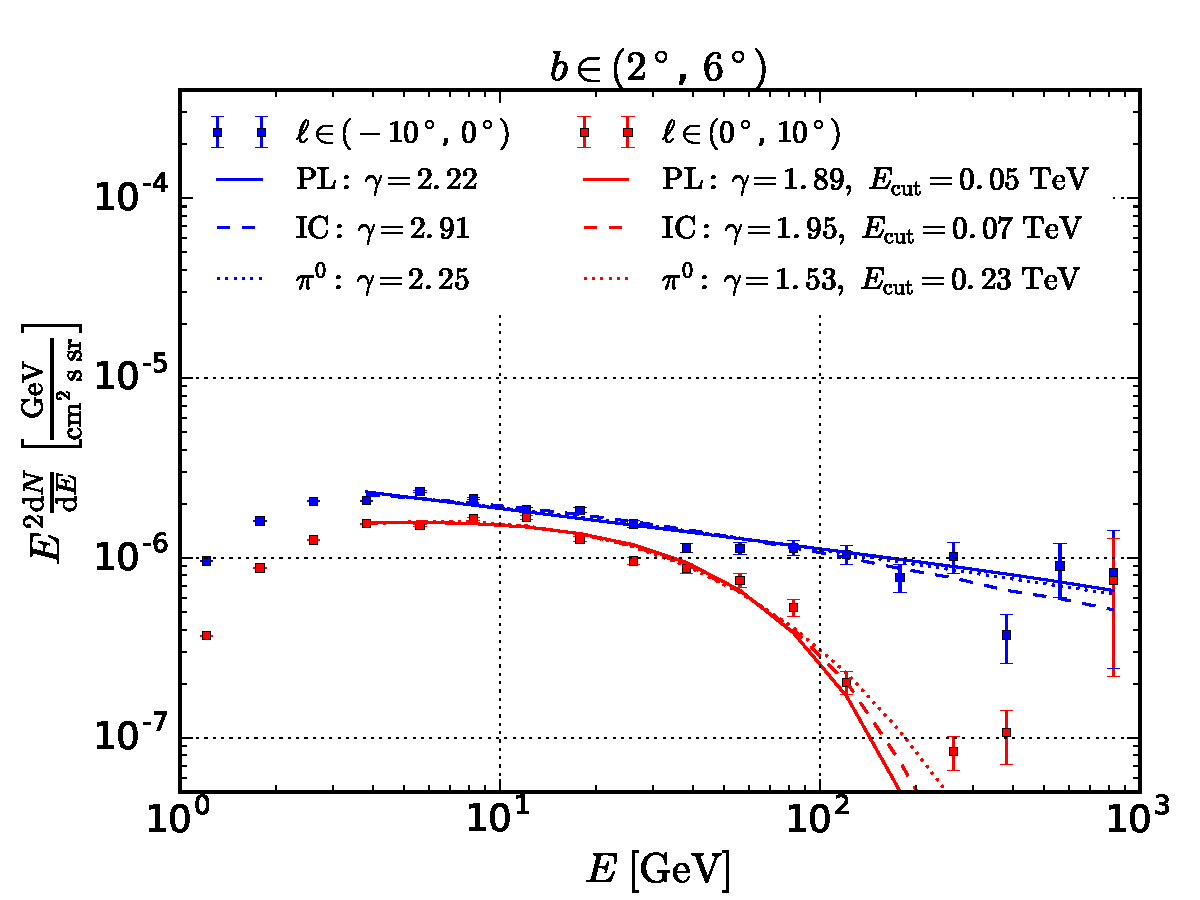
\includegraphics[width=0.33\textwidth]{plots/SED_boxes_source_4cutoff.pdf}
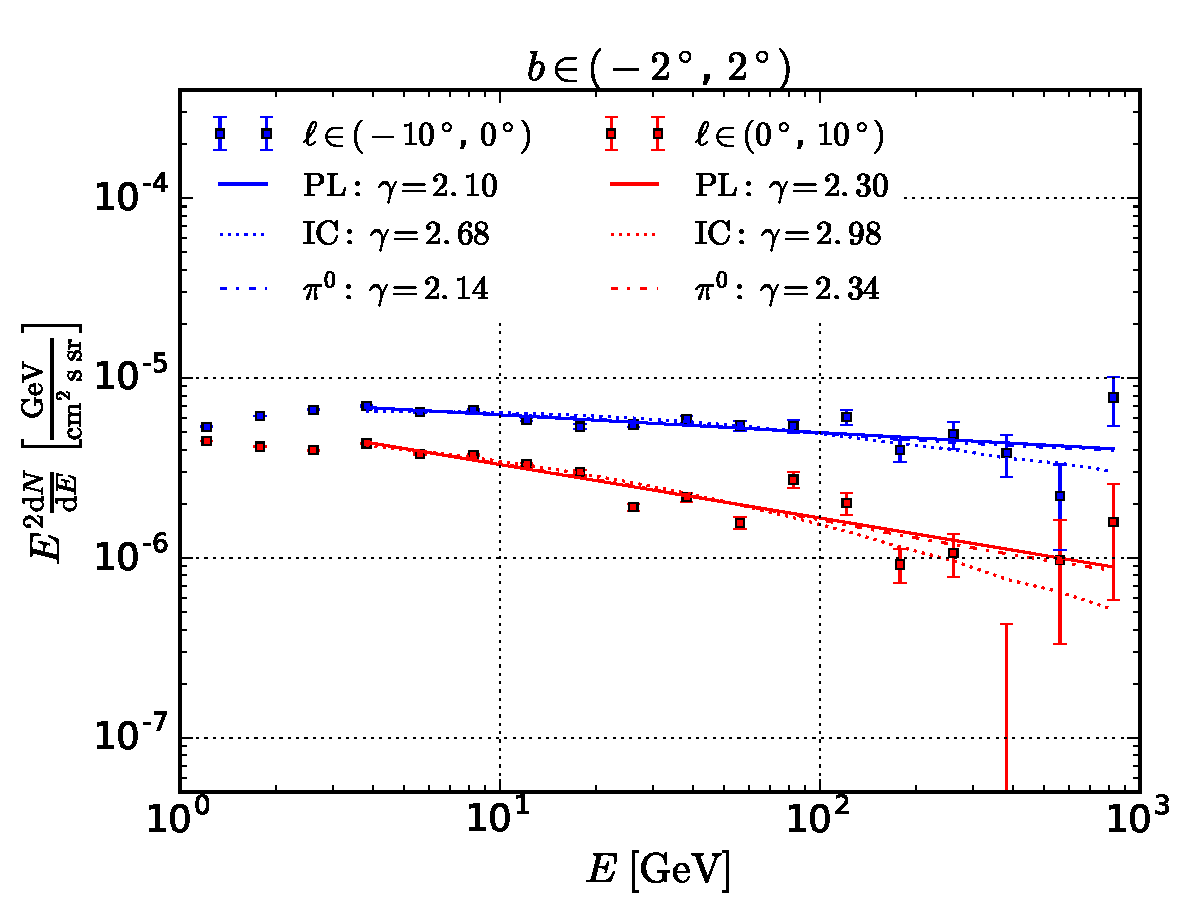
\includegraphics[width=0.33\textwidth]{plots/SED_boxes_source_0.pdf}
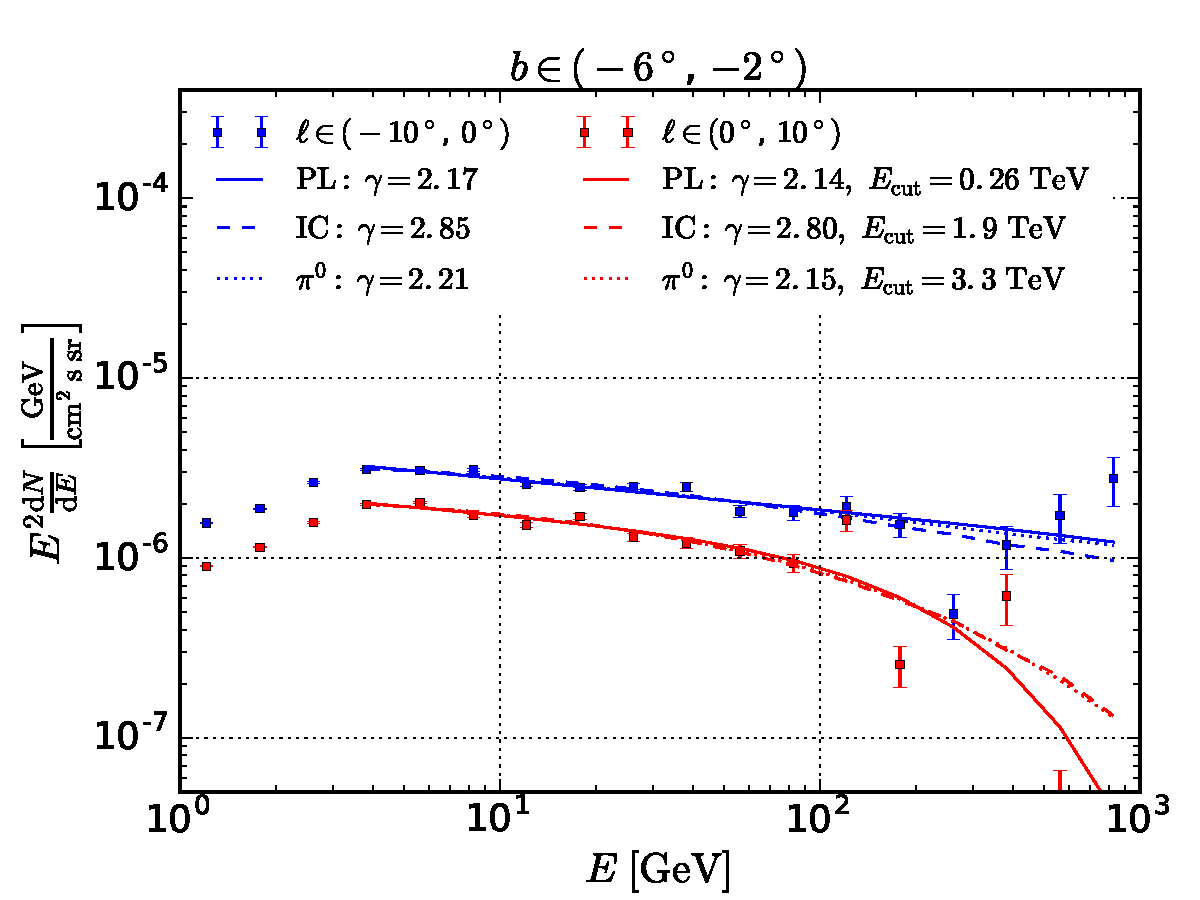
\includegraphics[width=0.33\textwidth]{plots/SED_boxes_source_-4cutoff.pdf}
%\end{comment}
% version for the two-column style?
\begin{comment}
    \begin{subfigure}{0.49\textwidth}
        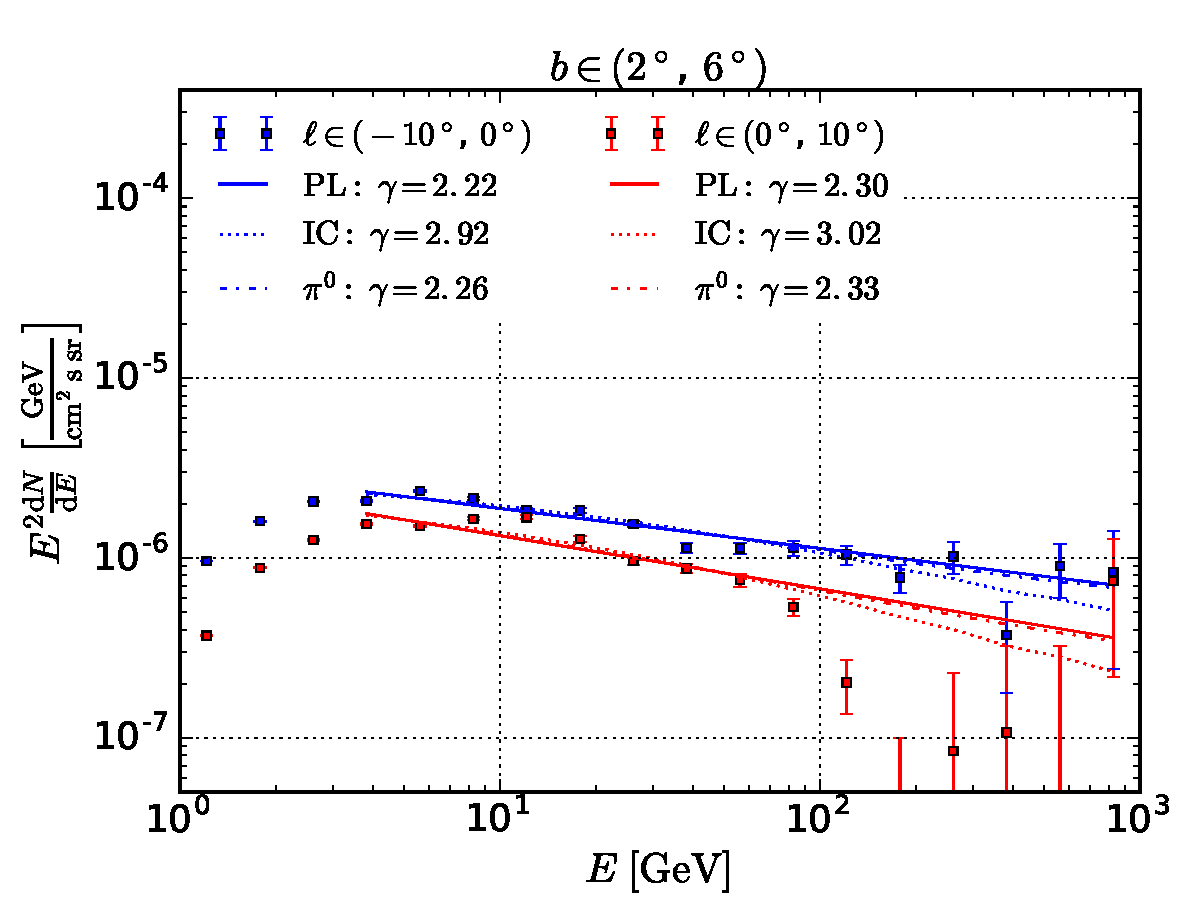
\includegraphics[width=\textwidth]{plots/SED_boxes_source_4.pdf}
    \end{subfigure}\\
    \begin{subfigure}{0.49\textwidth}
        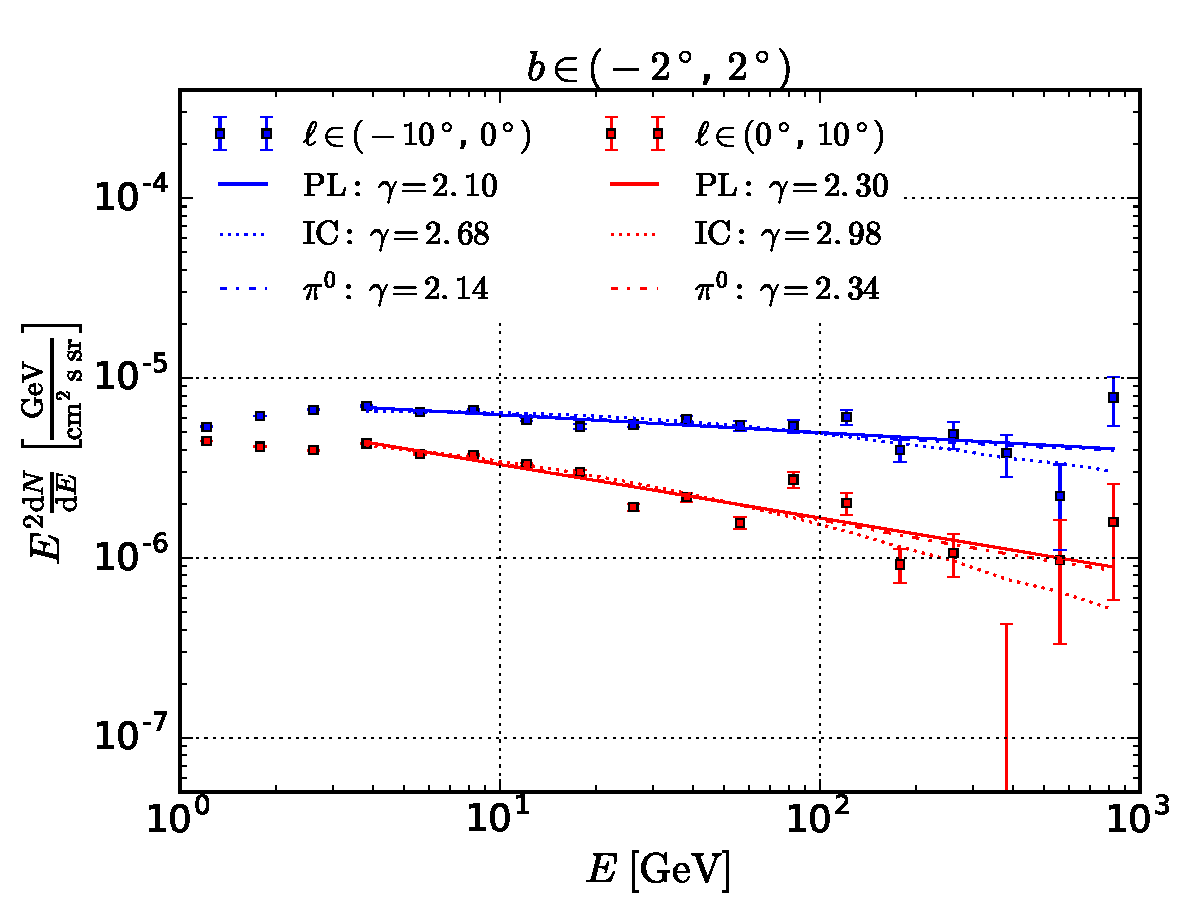
\includegraphics[width=\textwidth]{plots/SED_boxes_source_0.pdf}
    \end{subfigure} \\
    \begin{subfigure}{0.49\textwidth}
        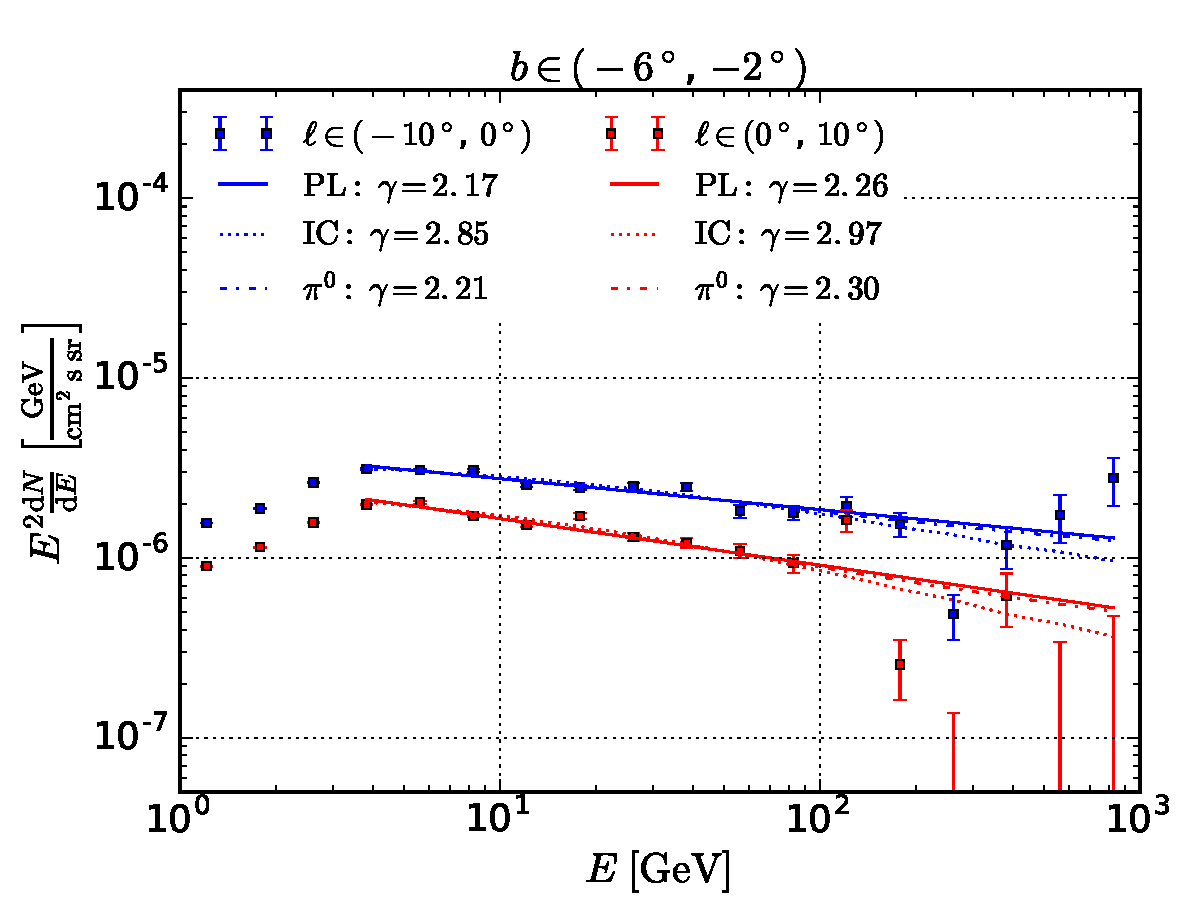
\includegraphics[width=\textwidth]{plots/SED_boxes_source_-4.pdf}
    \end{subfigure}
\end{comment}
  	\caption{SED of rectangles-model residual in the latitude stripes $(\ang{2}, \ang{6})$, $(\ang{-2}, \ang{2})$ and $(\ang{-6}, \ang{-2})$ for negative (blue) and positive (red) longitudes. We determine the spectral index of a powerlaw (PL), of an electron distribution emitting gamma-rays via IC and of a proton distribution emitting gamma-rays via $\pi^0$-decay.}
  	%\Laura{Should we add the spectrum for the latitude band $(\ang{2}, \ang{6})$ also, or just say that it looks similar?}
	%\blue{Dima: yes, let's add the 2 to 6 deg spectrum.}
  	\label{fig:SED_with_fits}
\end{figure*}

%
%\begin{center}
%\begin{tabular}{ |c|c|c|c|c| } 
% \hline
% lat & lon  & $\chi^2$(no cutoff) &  $\chi^2$(cutoff) & Lower bound $E_\cut$ \\ 
% \hline
%  2 -- 6 & east & $\chi^2$(no cutoff) &  $\chi^2$(cutoff) & Lower bound $E_\cut$\\ 
%2 -- 6 & west & $\chi^2$(no cutoff) &  $\chi^2$(cutoff) & Lower bound $E_\cut$ \\ 
% \hline
%   -2 -- 2 & east & $\chi^2$(no cutoff) &  $\chi^2$(cutoff) & Lower bound $E_\cut$\\ 
%-2 -- 2 & west & $\chi^2$(no cutoff) &  $\chi^2$(cutoff) & Lower bound $E_\cut$\\ 
% \hline
%  -6 -- -2 & east & $\chi^2$(no cutoff) &  $\chi^2$(cutoff) & Lower bound $E_\cut$\\ 
%-6 -- -2 & west & $\chi^2$(no cutoff) &  $\chi^2$(cutoff) & Lower bound $E_\cut$\\ 
% \hline
%\end{tabular}
%\end{center}

\begin{table*}
  \begin{center}
    \caption{Energy cutoff values and the significance of the cutoff in the IC model of the FB at low latitudes.
%  $\chi^2$-values for IC-spectrum fit of a distribution of electrons following a simple powerlaw and a powerlaw with cutoff, respectively in the latitude bands discussed in the text. 
The lower bounds for $E_\cut$ at the 95\% confidence level for our baseline model and the minimum among all
models are shown in the last two columns respectively.
}
    \label{tab:IC}
    \begin{tabular}{|c|c|c|c|c|} % <-- Alignments: 1st column left, 2nd middle and 3rd right, with vertical lines in between
     	\hline
		 Lat & Lon  & $-2 \Delta \log \La$ & \multicolumn{2}{c|}{Lower bound on $E_\cut$ (TeV) } \\ 
		       &        &                                  &  \multicolumn{1}{c}{Rectangles model} & All models \\ 
		\hline
  		$(\ang{2}, \ang{6})$ & $(\ang{0}, \ang{10})$ & 2.6  & 0.05 & 0.05 \\ 
		& $(\ang{-10}, \ang{0})$ & 0.0  & 4.0  & 4.0 \\ 
 		\hline
  		$(\ang{-2}, \ang{2})$ & $(\ang{0}, \ang{10})$ & 0.0 & 1.5 & 0.01 \\ 
		& $(\ang{-10}, \ang{0})$ & 0.0 & 13  & 2.9  \\ 
 		\hline
  		$(\ang{-6}, \ang{-2})$ & $(\ang{0}, \ang{10})$ & 1.1 & 0.83 & 0.03 \\ 
		& $(\ang{-10}, \ang{0})$& 0.0 & 6.3 & 6.3\\ 
 \hline
    \end{tabular}
  \end{center}
\end{table*}




%\begin{figure}
%	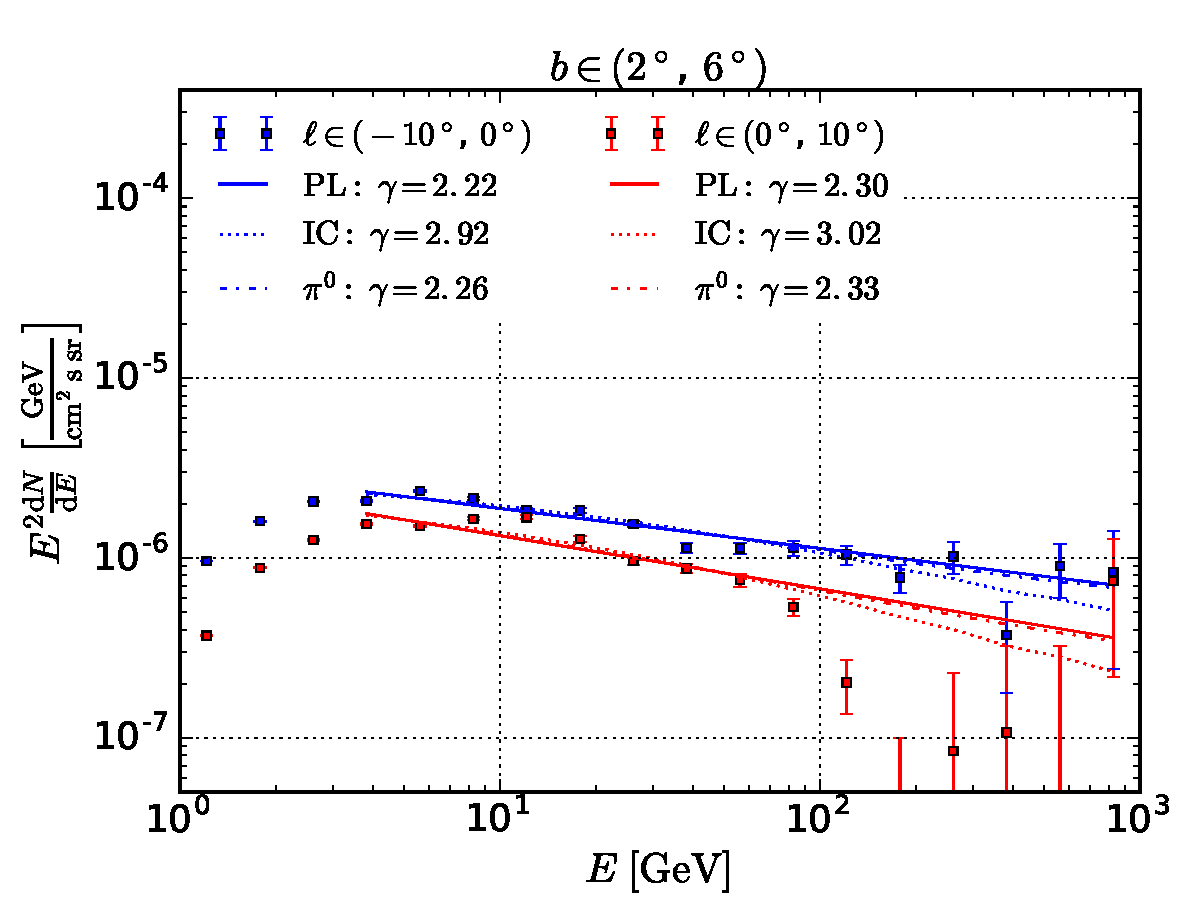
\includegraphics[width=0.5\textwidth]{plots/SED_boxes_source_4.pdf}
%\end{figure}
%\begin{figure}
%	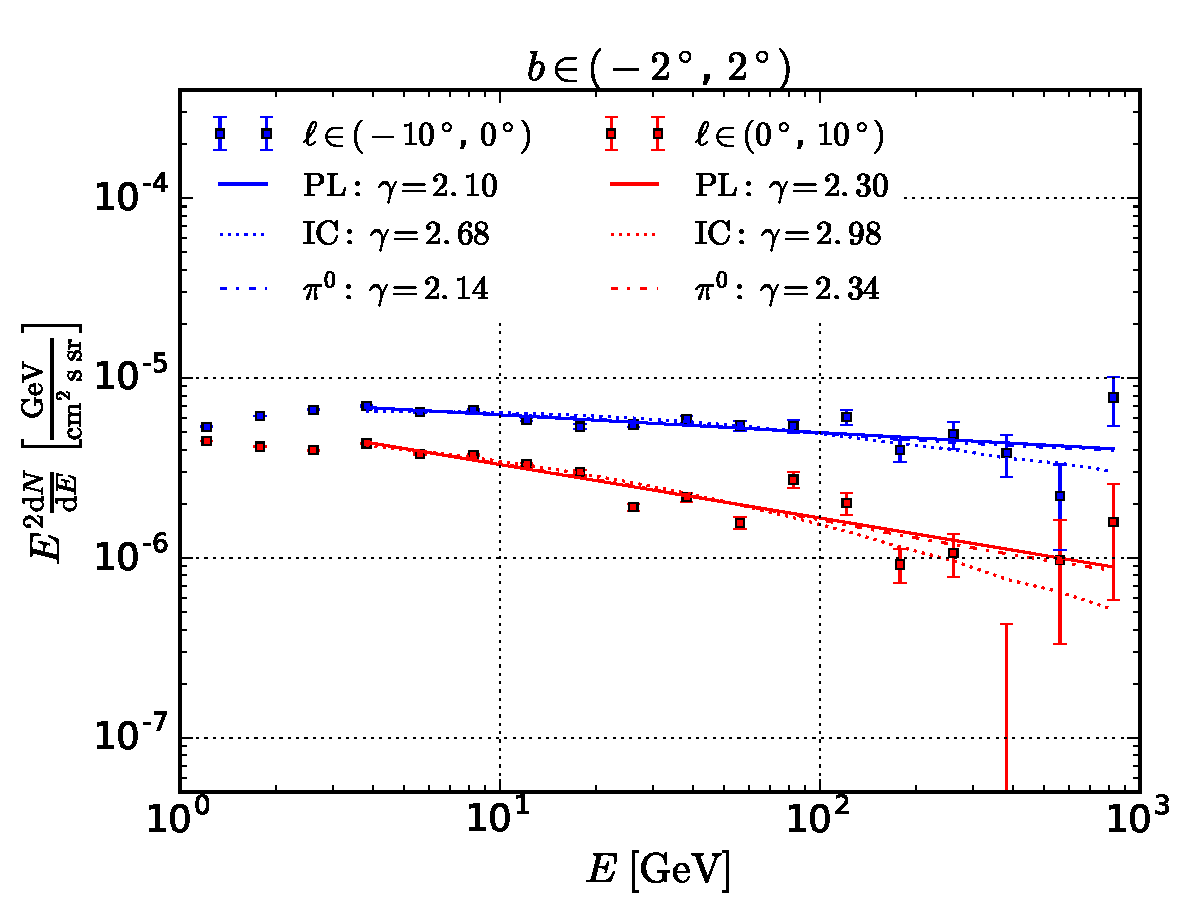
\includegraphics[width=0.5 \textwidth]{plots/SED_boxes_source_0.pdf}
%\end{figure}
%\begin{figure}
%	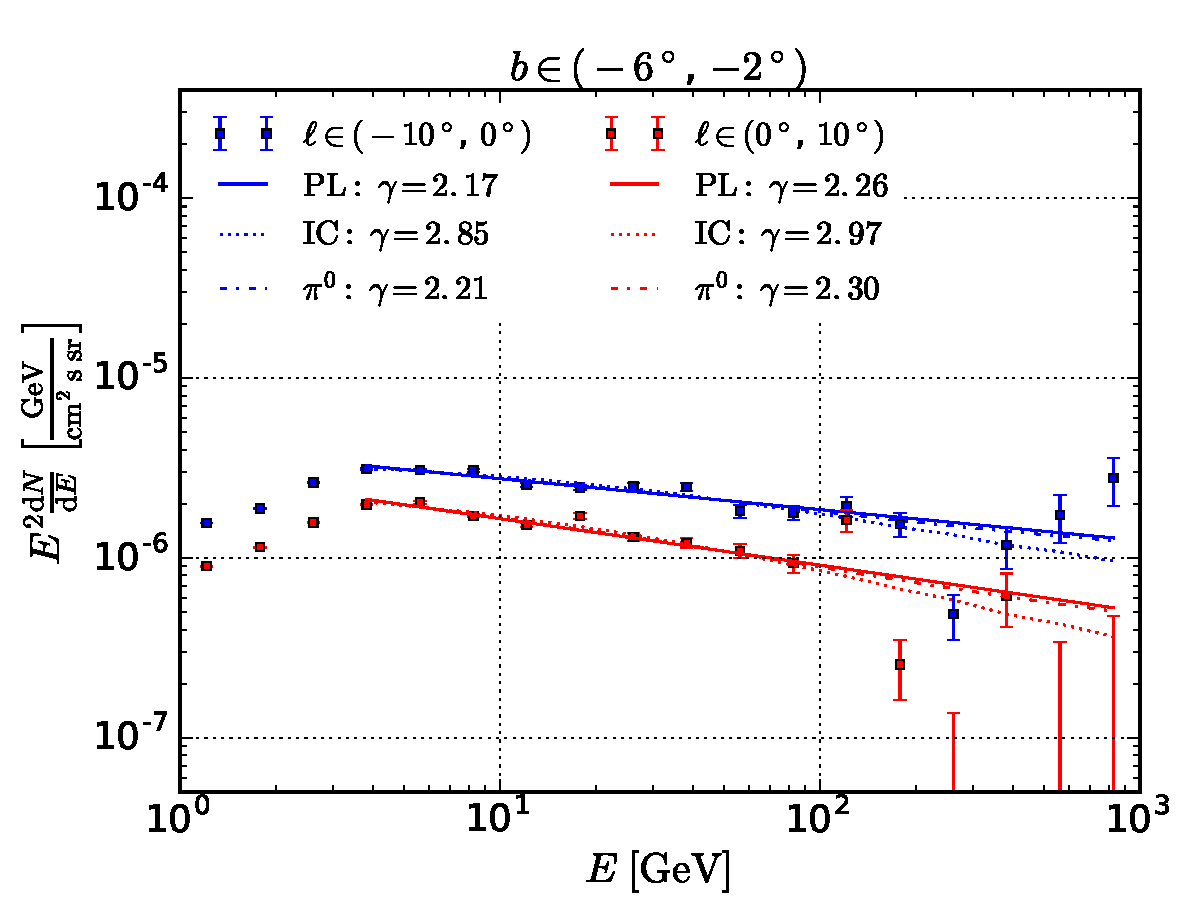
\includegraphics[width=0.5\textwidth]{plots/SED_boxes_source_-4.pdf}
%	\caption{SED of rectangles-model residual in the latitude stripes $(\ang{-2}, \ang{2})$ (left) and $(\ang{-6}, \ang{-2})$ (right) for negative (blue) and positive longitudes (red). We determine the spectral index of a powerlaw (PL), of an electron distribution emitting gamma-rays via IC and of a proton distribution emitting gamma-rays via $\pi^0$-decay.}
%\end{figure}


\subsection{Hadronic model of gamma-ray emission}
\label{sec:Pion_model}

In the hadronic model, the gamma rays are produced as a result of collisions of hadronic CR with the interstellar gas.
The source function for the gamma rays is 
\be
\left(E\frac{\de Q}{\de E}\right)_{\!\!\gamma, \pi^0}\! = \int n_\Hy\ \sigma_\pr v_\pr \left(\frac{\de n}{\de T}\right)_{\!\!\pr} \de T_\pr,
\label{eq:had_spectrum}
\ee
where the integral goes over the kinetic energies of the protons $T_\pr = \sqrt{(qc)^2 + (mc^2)^2} - mc^2$,
$n_\Hy$ is the density of gas, and $\sigma_\pr (E_\gamma, T_\pr)$ is 
the differential cross section in units of $E_\g\frac{d\sigma}{d E_\g}$
for gamma rays in proton-proton collisions \citep{2006ApJ...647..692K, 2008ApJ...674..278K}.
We will use $n_\Hy = \SI{1}{cm^{-3}}$ as a characteristic density,
which is consistent with the gas surface density of $\sim 10 M_\odot {\rm pc}^{-2}$ \citep{2017ApJ...834...57M}
averaged over $\approx 200$ pc above and below the GC.
The gamma-ray flux in the hadronic model is

\be
E^2 \frac{dF}{dE} = \frac{E}{4\pi} \int n_\Hy\ \sigma_\pr v_\pr \left(\frac{\de \Sigma}{\de T}\right)_{\!\!\pr} \de T_\pr,
%\frac{Ec}{4\pi}\int \int \left(\frac{\de n}{\de E}\right)_{\!\!\ISRF} \sigma_\IC\ \left(\frac{\de \Sigma}{\de E}\right)_{\!\!\el} \de E_\ISRF\, \de E_\el,
\ee
where $\left(\frac{\de \Sigma}{\de E}\right)_{\!\!\pr} = \int \left(\frac{\de n}{\de E}\right)_{\!\!\pr} dR$ is the column density 
of CR protons.
We will model the proton spectrum as a power law of the momentum $\frac{d \Sigma}{d qc} = n_\pr q^{-\g_p}$ 
(note, that $ v \frac{\de \Sigma}{\de T} = c \frac{d \Sigma}{d qc}$).

We add the hadronic model of the gamma-ray emission at the base of the FB to the foreground emission 
and determine the normalization $n_\pr$ and index $\gamma_\pr$ of the CRp spectrum
by fitting the total model to the \Fermi-LAT data using Poisson log likelihood.
The dash-dotted line in Figure \ref{fig:SED_with_fits} represents the best-fit hadronic spectrum (labeled as $\pi^0$). 
The index of the proton spectrum is relatively hard $\g_\pr \lesssim 2.3$, especially to the West of the GC.
\begin{comment}
For that, we again fit the sum of the photon counts generated by hadronic processes and the baseline model for the foreground to the total photon counts detected by the \Fermi-LAT (with PS mask) using Poisson likelihood.  
For $b \in (\ang{2}, \ang{6})$ the spectral index to the West of the GC varies between 2.26 and 2.42, for $b \in (-\ang{2}, \ang{2})$ between 2.14 and 2.64 and for $(-\ang{6}, -\ang{2})$ between 2.21 and 2.32. To the East of the GC the indices vary between 2.33 and 3.55. 
\end{comment}

We calculate the significance of a cutoff in the CRp spectrum by adding an exponential cutoff factor and refitting the model to the gamma-ray data.
The improvement in the model and the 95\% confidence lower bound on the cutoff values are presented in Table \ref{tab:pi0}.
Within $\pm 6^\circ$ from the Galactic plane West of the GC, the 95\% confidence level for the lower bound on the cutoff among all the models
of the foreground emission that we have considered is about 1.6 TeV.


\begin{comment}
We again estimate the probability for the proton spectrum to have an exponential cutoff: For the latitude stripe covering the Galactic plane, $b \in (-\ang{2}, \ang{2})$, adding a cutoff does neither improve the $\chi^2$-valueat negative ($\chi^2 \approx 62$) nor positive longitudes ($\chi^2 \approx 116$). At a $95\%$-confidence level, the lower bound for the cutoff energy for the baseline model (and all models) is $\SI{28.6}{TeV}$ ($\SI{22.6}{TeV}$) for negative longitudes and $\SI{1.8}{TeV}$ ($\SI{11.5}{GeV}$) for positive longitudes.\\
In the latitude band $(-\ang{6}, -\ang{2})$, the $\chi^2$-value does increase both for negative ($\chi^2 = 157$ to $\chi^2 = 123$) and positive longitudes ($\chi^2 = 245$ to $\chi^2 = 156$) by adding an exponential cutoff. The lower bound on the cutoff energy is $\SI{23.6}{TeV}$ ($\SI{0.99}{TeV}$) for negative and $\SI{1.57}{TeV}$ ($\SI{40}{GeV}$) for positive longitudes.
\end{comment}


\begin{table*}
  \begin{center}
    \caption{\label{tab:pi0} 
Energy cutoff values and the significance of the cutoff in the hadronic model of the FB at low latitudes.
%    $\chi^2$-values for hadronic-spectrum fit of a distribution of protons following a simple powerlaw and a powerlaw with a cutoff, respectively in the latitude bands discussed in the text. 
The lower bounds for $E_\cut$ at the 95\% confidence level for our baseline model and the minimum among all
models are shown in the last two columns respectively. 
}
    \begin{tabular}{|c|c|c|c|c|} % <-- Alignments: 1st column left, 2nd middle and 3rd right, with vertical lines in between
     	\hline
		 lat & lon  & $-2 \Delta \log \La$ & \multicolumn{2}{c|}{Lower bound on $E_\cut$ (TeV) } \\
		      &        &                                  &       \multicolumn{1}{c}{Rectangles model} & All models \\ 
		\hline
  		$(\ang{2}, \ang{6})$ & $(\ang{0}, \ang{10})$ & 4.4 & 0.16  & 0.16 \\ 
		& $(\ang{-10}, \ang{0})$ &  0.0 & 1.6 & 1.6 \\ 
 		\hline
  		$(\ang{-2}, \ang{2})$ & $(\ang{0}, \ang{10})$ & 0.0 & 1.3 & 0.023 \\ 
		& $(\ang{-10}, \ang{0})$ & 0.0 & 30 & 6.3 \\ 
 		\hline
  		$(\ang{-6}, \ang{-2})$ & $(\ang{0}, \ang{10})$ & 2.7 & 1.6 & 0.05 \\ 
		& $(\ang{-10}, \ang{0})$ & 0.0 & 2.1 & 2.1 \\ 
 \hline
    \end{tabular}
  \end{center}
\end{table*}

\subsection{Summary of the spectral analysis}

In Figure \ref{fig:spec_summary} we show the envelopes of the gamma-ray spectra at $|b| < 2^\circ$ of the residuals including
the FB for the different models of the foreground emission including the changes in the selection of the low energies 
in the definition of the foreground emission model (Appendix \ref{sec:lowE_syst}).
In order to determine the maximal and minimal models of the FB in the Galactic plane, 
we fit above 3 GeV the maximal and minimal points in the envelope with a power-law and a cutoff function.
The corresponding parameters are reported in the first raw of Table \ref{tab:summary}.
We also fit the IC and hadronic models to the maximal and minimal points in the envelope and report the corresponding parameters
in Table \ref{tab:summary}.


%\dima{we can put a summary plot with the baseline model and the band of all spectra in a small subsection here}

\begin{figure}[h]
\centering
 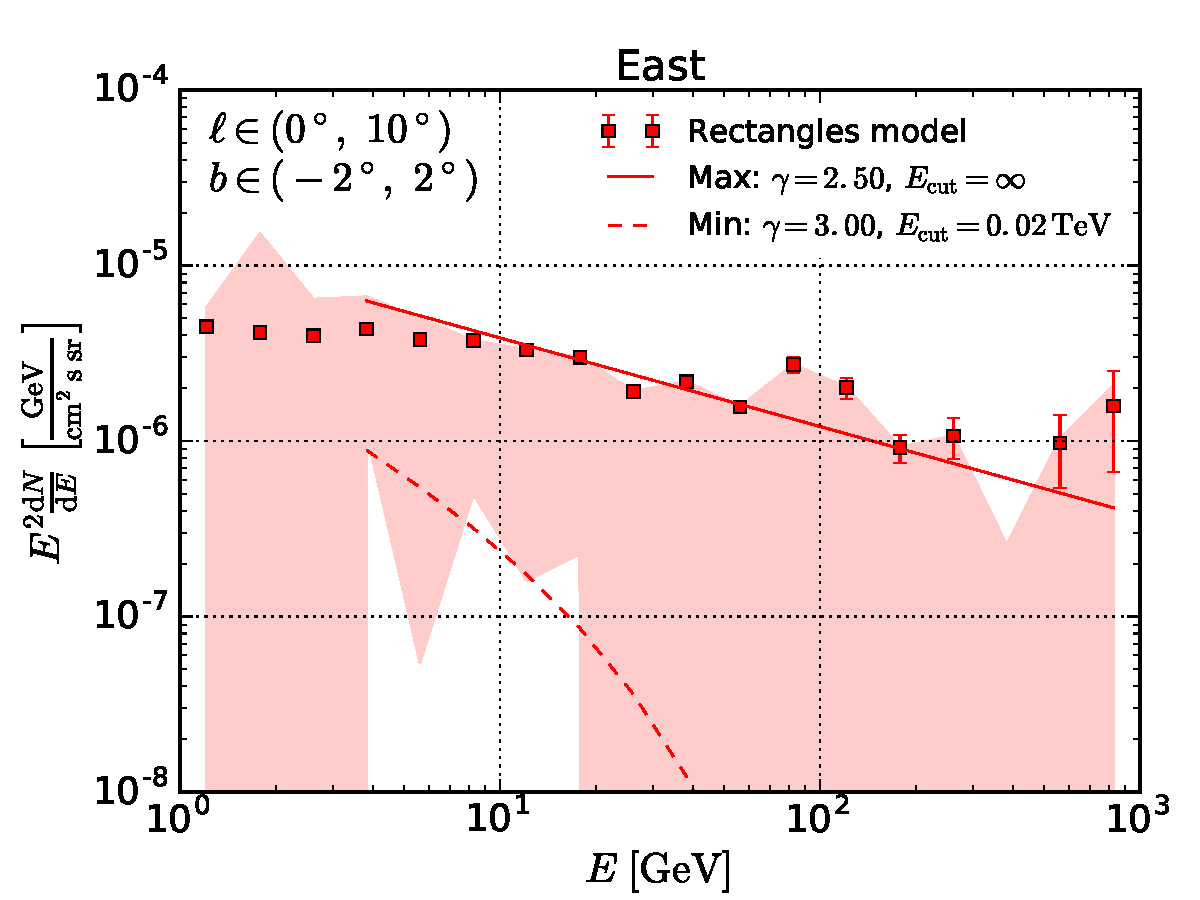
\includegraphics[width=0.48\textwidth]{plots/Summary_SED_b=0_l=5.pdf}
  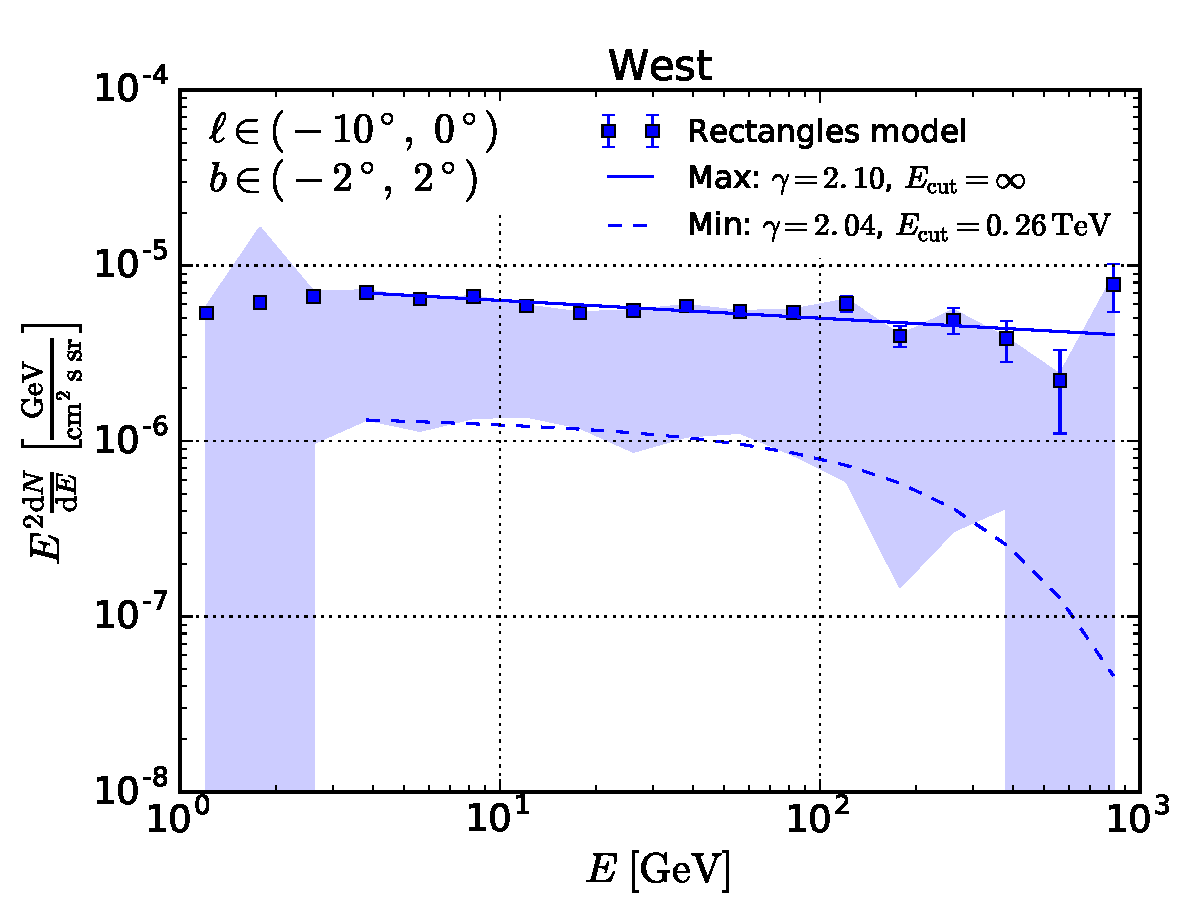
\includegraphics[width=0.48\textwidth]{plots/Summary_SED_b=0_l=-5.pdf}
 \caption{SED of the FB in the Galactic plane. 
 The shaded areas show the envelope of the FB spectra in all foreground models considered in the paper
including the changes in the choice of the low-energy range to model the foreground emission
(discussed in Appendix \ref{sec:lowE_syst}).}
 \label{fig:spec_summary}
\end{figure}


\begin{table*}
  \begin{center}
    \caption{Summary of the min and max models for the parametric, 
    IC and hadronic models of the FB for $|b| < 2^\circ$ and $-10^\circ < \ell < 0^\circ$. 
    For the parametric model we report the energy spectrum of the gamma rays,
    for the IC model we report the surface density of the electrons spectrum as a function of energy,
    while for the hadronic model -- the surface density of the protons spectrum as a function of momentum.
    The spectra are normalized at $E_0 = 1$ GeV.}
    \label{tab:summary}
    \begin{tabular}{| l |c|c|c|c|c|c|c|} % <-- Alignments: 1st column left, 2nd middle and 3rd right, with vertical lines in between
     	\hline
		 {\hspace{2cm}Model} & Type  & norm & index & cutoff & cutoff 95\% stat \\ 
		       &        &   &  & {\rm TeV} & {\rm TeV}\\ 
		\hline
  		\multirow{2}{*}{Parametric, $\frac{dN_\g}{dE} = \left[{\rm \frac{1}{GeV\, cm^{2}\, s}}\right]$} & max & $\SI{8.0e-6}{}$  & 2.1 &  -- & 3.9 \\ 
		& min & $\SI{1.4e-6}{}$ & 2.0 &  0.26 & 0.14  \\ 
 		\hline
  		\multirow{2}{*}{IC, $\frac{d\Sigma_e}{dE} = \left[{\rm \frac{1}{GeV\, cm^2}}\right]$}& max & $\SI{1.8e10}{}$  & 2.7 &  -- & 60 \\ 
		& min & $\SI{2.5e9}{}$  & 2.6 &  1.1 & 0.4  \\ 
 		\hline
  		\multirow{2}{*}{Hadronic, $\frac{d\Sigma_p}{dqc} = \left[{\rm \frac{1}{GeV\, cm^2}}\right]$} & max & $\SI{4.4e11}{}$  & 2.1 &  -- & 270 \\ 
		& min & $\SI{4.9e10}{}$  & 2.0 &  2.3 & 1.1  \\ 
 \hline
    \end{tabular}
  \end{center}
\end{table*}



